%! Author = chtompki
%! Date = 1/14/26
% Example LaTeX document for GP111 - note % sign indicates a comment
\documentclass[12pt]{amsart}
% Default margins are too wide all the way around. I reset them here
\setlength{\hoffset}{-.75in}
\setlength{\textwidth}{6.5in}
\setlength{\voffset}{-.5in}
\setlength{\textheight}{9.0in}
\usepackage{amsmath}
\usepackage{amssymb}
\usepackage{amsthm}
\usepackage{pgfplots}
\usepackage{enumerate}
\usepackage{tikz}
\usetikzlibrary{shadows,arrows,arrows.meta,shapes,positioning,calc}% Required for the Circle and Triangle arrow tips
\usepackage{setspace}
\usepackage{siunitx}

\theoremstyle{definition}
\newtheorem{definition}{Definition}

\theoremstyle{question}
\newtheorem{question}{Question}

\title{Seminar Summary:\\March 31, 2026 - Neal Bushaw\\Bootstrap percolation on grids.}
\author{Rob Tompkins}
\date{\today}


\begin{document}
    \maketitle
    \date{\today}
    \begin{onehalfspace}
        Percolation theory is a branch of mathematics rooted in time based graphical
        shading changes related to a set of rules and an initial condition.
        We were presented with an $n\times m$ square tiling of the plane.
        Our initial condition was a collection of shaded blocks, take Figure \ref{m_n_grid_5filled}
        for example.
        The percolating mechanic was then set to being that if a square has $k$ shaded (or infected)
        neighbors then in the next time step, it will become shaded, and time steps in definite intervals.
        For example, if $k=1$, the behaviour is as if each square becomes a ``source'' in the sense of water
        or sand, and over time the entire board is filled so long as there is a single shaded block
        at our initial condition.

        \begin{figure}
            \begin{tikzpicture}[scale=1]

                % Dimensions
                \def\rows{4}
                \def\cols{5}

                % Draw all cells explicitly (ensures borders everywhere)
                \foreach \i in {0,...,4} {
                    \foreach \j in {0,...,3} {
                        \draw (\i,\j) rectangle (\i+1,\j+1);
                    }
                }

                % Shade selected cells
                \fill[black!25] (0,3) rectangle (1,4); % (1,1)
                \fill[black!25] (2,3) rectangle (3,4); % (1,3)
                \fill[black!25] (0,2) rectangle (1,3); % (2,1)
                \fill[black!25] (3,2) rectangle (4,3); % (2,4)
                \fill[black!25] (3,0) rectangle (4,1); % (m,4)

                % Redraw borders on top of shading (important!)
                \foreach \i in {0,...,4} {
                    \foreach \j in {0,...,3} {
                        \draw (\i,\j) rectangle (\i+1,\j+1);
                    }
                }

                % Column labels
                \node at (0.5,4.3) {$1$};
                \node at (1.5,4.3) {$2$};
                \node at (2.5,4.3) {$3$};
                \node at (3.5,4.3) {$\cdots$};
                \node at (4.5,4.3) {$n$};

                % Row labels
                \node[left] at (-0.2,3.5) {$1$};
                \node[left] at (-0.2,2.5) {$2$};
                \node[left] at (-0.2,1.5) {$\vdots$};
                \node[left] at (-0.2,0.5) {$m$};

                % Label underneath
                \node at (2.5,-0.6) {$G_{4,5}$};
            \end{tikzpicture}
            \caption{A rectangular $G_{4,5}$ tiled with squares, five shaded as bootstrap for percolation.}
            \label{m_n_grid_5filled}
        \end{figure}

        We then began looking at the scenario for $k=2$ (i.e. two neighbors, as edge neighbors, not corner neighbors).
        If we were to take Figure \ref{m_n_grid_5filled}, and step it once in time, then we would get Figure \ref{m_n_grid_8filled}.

        \begin{figure}
            \begin{tikzpicture}[scale=1]

                % Dimensions
                \def\rows{4}
                \def\cols{5}

                % Draw all cells explicitly (ensures borders everywhere)
                \foreach \i in {0,...,4} {
                    \foreach \j in {0,...,3} {
                        \draw (\i,\j) rectangle (\i+1,\j+1);
                    }
                }

                % Original shaded cells
                \fill[black!25] (0,3) rectangle (1,4); % (1,1)
                \fill[black!25] (2,3) rectangle (3,4); % (1,3)
                \fill[black!25] (0,2) rectangle (1,3); % (2,1)
                \fill[black!25] (3,2) rectangle (4,3); % (2,4)
                \fill[black!25] (3,0) rectangle (4,1); % (m,4)

                % NEW shaded cells
                \fill[black!25] (1,3) rectangle (2,4); % (1,2)
                \fill[black!25] (2,2) rectangle (3,3); % (2,3)
                \fill[black!25] (3,1) rectangle (4,2); % (3,4)


                % Redraw borders on top of shading (important!)
                \foreach \i in {0,...,4} {
                    \foreach \j in {0,...,3} {
                        \draw (\i,\j) rectangle (\i+1,\j+1);
                    }
                }

                % Column labels
                \node at (0.5,4.3) {$1$};
                \node at (1.5,4.3) {$2$};
                \node at (2.5,4.3) {$3$};
                \node at (3.5,4.3) {$\cdots$};
                \node at (4.5,4.3) {$n$};

                % Row labels
                \node[left] at (-0.2,3.5) {$1$};
                \node[left] at (-0.2,2.5) {$2$};
                \node[left] at (-0.2,1.5) {$\vdots$};
                \node[left] at (-0.2,0.5) {$m$};

                % Label underneath
                \node at (2.5,-0.6) {$G_{4,5}$};
            \end{tikzpicture}
            \caption{A rectangular $G_{4,5}$ tiled with squares, eight shaded after time step 1 with $k=2$.}
            \label{m_n_grid_8filled}
        \end{figure}
        Eventually this initial value percolation from Figures \ref{m_n_grid_5filled} and \ref{m_n_grid_8filled}
        fills the entire space except for the right column of squares.
        Oddly some of these bootstrap percolations fill the entire space, some leave just edges behind, and some stop entirely.
        The goal behind the research here is to classify the different categories of initial conditions.

        We then explored a considerable number of different bootstraps (or initial conditions) randomdomly
        generated for the $k=2$ problem.
        It was interesting to see which percolated to the entire domain and which stopped.
        Figure \ref{m_n_grid_steady_state} gives us this steady state where percolation cannot continue.
        \begin{figure}
            \begin{tikzpicture}[scale=0.35]

                % Grid size
                \def\rows{19}
                \def\cols{37}

                % Helper: shade cell at row r, column c
                % Rows counted from top, columns from left
                \newcommand{\shadecell}[2]{%
                    \fill[gray!65] ({#2-1},{\rows-#1}) rectangle ({#2},{\rows-#1+1});
                }

                % ---- shaded cells ----

                % row 1
                \shadecell{1}{31}

                % row 2
                \shadecell{2}{5}
                \shadecell{2}{18}
                \shadecell{2}{27}
                \shadecell{2}{28}
                \shadecell{2}{29}

                % row 3
                \shadecell{3}{9}
                \shadecell{3}{10}
                \shadecell{3}{11}
                \shadecell{3}{12}
                \shadecell{3}{13}
                \shadecell{3}{27}
                \shadecell{3}{28}
                \shadecell{3}{29}

                % row 4
                \shadecell{4}{9}
                \shadecell{4}{10}
                \shadecell{4}{11}
                \shadecell{4}{12}
                \shadecell{4}{13}

                % row 5
                \shadecell{5}{2}

                % row 6
                \shadecell{6}{5}

                % row 7
                \shadecell{7}{13}
                \shadecell{7}{14}
                \shadecell{7}{33}

                % row 8
                \shadecell{8}{37}

                % row 9
                \shadecell{9}{22}

                % row 10
                \shadecell{10}{15}
                \shadecell{10}{26}

                % row 11
                \shadecell{11}{5}
                \shadecell{11}{10}
                \shadecell{11}{15}

                % row 12
                \shadecell{12}{2}
                \shadecell{12}{3}
                \shadecell{12}{15}
                \shadecell{12}{36}

                % row 13
                \shadecell{13}{7}

                % row 14
                \shadecell{14}{7}
                \shadecell{14}{14}
                \shadecell{14}{22}

                % row 15
                \shadecell{15}{7}
                \shadecell{15}{34}

                % row 16
                \shadecell{16}{9}
                \shadecell{16}{30}

                % row 17
                \shadecell{17}{11}
                \shadecell{17}{15}
                \shadecell{17}{19}
                \shadecell{17}{22}

                % row 18
                \shadecell{18}{2}
                \shadecell{18}{19}
                \shadecell{18}{26}
                \shadecell{18}{31}

                % Draw all cell borders explicitly
                \foreach \x in {0,...,36} {
                    \foreach \y in {0,...,18} {
                        \draw[black] (\x,\y) rectangle (\x+1,\y+1);
                    }
                }

                % Outer border slightly thicker
                \draw[line width=0.8pt] (0,0) rectangle (\cols,\rows);

            \end{tikzpicture}
            \caption{A large square based Bootstrap Percolation with $k=2$ in a steady state}
            \label{m_n_grid_steady_state}
        \end{figure}
        A question was then asked: what is the minimal number of squares needed filled such that
        a $k=2$ completely percolates to the entire domain.
        The answer curiously was that it need be a single diagonal from a corner to the other corner,
        for the square grid case.
        Take for example the identity matrix as an example.

        We then switched our attention to the square bootstrap percolation with $k=3$, and we
        found it much more difficult to get a percolation to the entire domain as there were
        far more stable configurations of squares.
        Furthermore, there was some subtle research going on about $k=3$ as recently as 2023 and 2025.

        Finally, we were presented with a variety of general tools for approaching the problem.

        Generally the problem seemed to garner quite a good amount of attention and engagement
        from the class which was fun.
        The problem itself seemed intuitive to follow at first, and then when $k$ was varied
        intuition was completely lost, making the problem different and interesting.
        A question was asked about applicability, and Professor Bushaw said that
        he was not concerned with application merely the curiosity of the problem which
        was interesting in its own right.
        It was definitely a problem that I could find myself exploring because I have
        a background in tilings over infinite words on the $n$ letter alphabet, but
        I do not know if that outweighs my interest in pure logic.
    \end{onehalfspace}
\end{document}
